\title{Appendices}

\documentclass[12pt]{article}
\usepackage{amsmath}
\usepackage{mathabx}
\usepackage{graphics}
\usepackage[top=0.75in, bottom=0.75in, left=1in, right=1in]{geometry}
\usepackage{tabu}
\usepackage[english]{babel}
\usepackage{natbib}
\bibliographystyle{evolution}
\usepackage{rotating}
\usepackage[capitalize, sort&compress]{cleveref}
\usepackage{float}
%\newcommand{\crefrangeconjunction}{--}
%\crefname{section}{Sect.}{Sects.}
%\crefname{equation}{Eq.}{Eqs.}
%\crefformat{equation}{Eq.~#2#1#3}
%\crefrangeformat{equation}{Eqs.~#3#1#4--#5#2#6}
%\crefmultiformat{equation}{Eqs.~#2#1#3}{--#2#1#3}{, #2#1#3}{ and~#2#1#3}
 
% for comments visible in the compiled pdf
%\usepackage{color}
%\definecolor{orange}{rgb}{0.8,0.4,0}
%\newcommand{\eeg}[1]{{\em \color{orange} #1}}

% Tell latex how it can introduce linebreaks if necessary.
\hyphenation{Bar-thol-o-mew}

\begin{document}
\maketitle 

\section{Sun movement}
\section*{Solar radiation: SR}
As in \citet{Campbell2012}, we model zenith angle ($\psi$) at time $t$ as
\begin{equation}  \label{eq:psi}
\cos(\psi) = \sin(\phi) \sin(\delta) + \cos(\phi) \cos(\delta) \cos[15 (t- t_0)] 
\end{equation}
Here, $\phi$ denotes latitude, $\delta$ denotes solar declination which varies between 23.45$^\circ$ and  -23.45$^\circ$ at summer and winter solstice 
($\delta$ as in equation 11.2 in \citet{Campbell2012} and only depends of the day of the year). 
$t_0$ represents the time of solar noon and since we do not span across longitude, we fix $t_0 = 12$.
For simplicity, we assume that solar radiation is \[SR = S_0 \cos(\psi) \] where $S_0 = 1361 \mbox{W.m}^{-2}$. 
\cref{fig:rad} shows variations of SR at different latitudes during solstice and equinox.

%\begin{figure}
%\begin{center}
%	\scalebox{0.75}{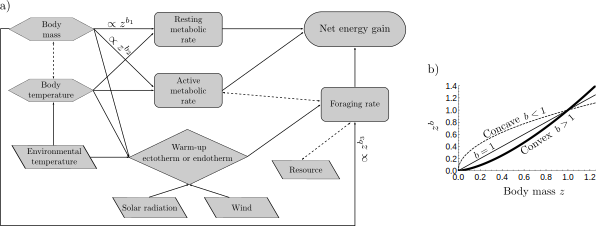
\includegraphics{fig1}}
%	\caption{Change in solar radiation during the course of the day at different latitudes---color coded and labeled numbers. 
%	Northern latitudes are denoted by positive numbers.  
%	}
%	\label{fig:rad}
%\end{center}
%\end{figure}

\section{Geometric property of the body}
$A_r$ which is the surface of the rest of the body is just total body surface.
We assume it is a half-a-sphere.
Knowing body mass $z$ and density $d$, we can convert mass into volume $ V = z/d$.
Then, we find the radius $r = [(3V)/(2 \pi)]^{1/3}$ (only half volume hence 2/3 not 4/3).
The body surface is   $A_r = 3 \pi r^2$ and the thoracic surface (assumed to be a quarter of a sphere) is $A_{th} = 2 \pi r^2$. 

The volume of a spherical cap is $V_{cap} = \frac{\pi h^2}{3} (3 r - h)$ where $h$ is the height of the cap (should be divided by 2)
The curved surface area of the spherical cap is $A_{curv} = 2 \pi r h$ where r is the radius. (Should be divided by two because it is a half a sphere)
The are of the circular segment is $A_{seg}= r^2 \cos^{-1} \left( \frac{r -h}{r}\right) - (r- h) \sqrt{2 r h - h^2}$. 
The total area of the thorax is $A_{th} = A_{curv} / 2 + A_{seg} \times 2$. 

The volume of the rest of the body is then $V_{rest} = \frac{2}{3} \pi r^3  - V_{cap} /2$.
The surface of the rest of the body is $A_{rest} = A_{s} = (4 \pi r^2 - A_{curv})/2 +   r^2 \pi $.

If $h$ is the height of the cap then the mass ratio between the thorax and the total body is $cz  = \frac{h^2 (3 r - h)}{4 r^3 }$ .

\section{Derivation of inequalities}
The daily net energy gain is the difference between energy collected $e_g$ during a period $t_f$ and the energy used during day partitioned as: energy for warm-up $e_w$, energy expended to acquire the resource $e_a$, and the resting metabolic energy $e_b$. 
For brevity, we omit the subscript of $z_b$. 
To start, let's assume that the ambient temperature is constant (i.e., $\alpha = 0$),

ADJUST  Q10 by multiplying by T0
\begin{flalign*}
	e_n(z) & = e_g(z) \times t_f  - \left( e_w(z)  + e_a(z) \times t_f + e_b(z) \times (3600\times 24 - t_f - t_w) \right) \\
			&  = \varepsilon a_3 z^{b_3} \times t_f  - \left( e_w(z)  + \rho a_1 z^{b_2} Q_{10}^{\frac{\tau}{10}} \times t_f +  a_1 z^{b_1} Q_{10}^{\frac{\tau}{10}} \times (3600\times24 - t_f - t_w) \right) 
\end{flalign*}

\subsubsection*{Case 1 = No warm-up}
For simplicity let us assume that there is no need to warm-up so that $e_w = 0 $ and $t_w =  0$.
\begin{flalign*}
	e_n(z) & = \varepsilon a_3 z^{b_3} \times t_f  - \left( \rho a_1 z^{b_2} Q_{10}^{\frac{\tau}{10}} \times t_f +  a_1 z^{b_1} Q_{10}^{\frac{\tau}{10}}\times (3600\times24 - t_f) \right) \\
			& =  z_3^{b_3} \left[  \varepsilon a_3 \times t_f  - \rho a_1 Q_{10}^{\frac{\tau}{10}} z^{b_2 - b_3} \times t_f -  a_1 z^{b_1- b_3} Q_{10}^{\frac{\tau}{10}}\times (3600\times24 - t_f) \right] 
%			& =  z_3^{b_3} \left[  (\varepsilon a_3  - \rho a_1 Q_{10}^{\frac{\tau}{10}} z^{b_2 - b_3}) \times t_f -  a_1 z^{b_1- b_3} Q_{10}^{\frac{\tau}{10}}\times (3600\times24 - t_f) \right] 
\end{flalign*}
Thus, the net energy gain is positive if the term between the square brackets is positive, 
\begin{flalign*}
	\varepsilon a_3 &> \rho a_1 Q_{10}^{\frac{\tau}{10}} z^{b_2 - b_3} +  a_1 z^{b_1- b_3} Q_{10}^{\frac{\tau}{10}}\times (3600 \times24 - t_f)/t_f \\
					    & >  \rho a_1 Q_{10}^{\frac{\tau}{10}} z^{b_2 - b_3}+  a_1 z^{b_1- b_3} Q_{10}^{\frac{\tau}{10}}\times 3600\times 24 /t_f -  a_1 z^{b_1- b_3} Q_{10}^{\frac{\tau}{10}} \\
					    & >  a_1 Q_{10}^{\frac{\tau}{10}} z^{b_2 - b_3} \left[  \rho+  \frac{3600\times24} {t_f} z^{b_1 - b_2}  - z^{b_1 - b_2}   \right]
\end{flalign*}
We denote $b_2 = b_1 + \nu_1$ with $\nu_1 \geq 0$, and $b_3 = b_1 + \nu_2$ where $\nu_2$ can be both negative and positive.
Therefore $b_3 = b_2 + (\nu_2 - \nu_1)$, abd 
\begin{equation}
	\varepsilon a_3 > a_1 Q_{10}^{\frac{\tau}{10}} z^{\nu_1 - \nu_2} \left[  \rho + \frac{3600\times24/t_f - 1}{z^{\nu_1}} \right]
\end{equation}
or 
\begin{equation}
	\frac{\varepsilon a_3}{Q_{10}^{\frac{\tau}{10}}} > a_1  z^{\nu_1 - \nu_2} \left[  \rho + \frac{3600\times24/t_f - 1}{z^{\nu_1}} \right]
\end{equation}

%\input{./Appendix_warm-up_derivation.tex }
\newpage

\bibliography{ref2}
\end{document}
